\chapter{INSTRUMENTATION SECTION}

\onehalfspacing

It is often said that the proliferation of knowledge and the accelerating development of technology 
have rendered our environment so complex that no one can understand even a small portion of it. 
The statement would have been undoubtly correct except for the circumstance that new knowledge can 
be better organized and that automation can relieve us of a considerable number of chores, as a
consequence of which activity can be concentrated on subjects having technological meaning. 

\vspace{1em}

In this evolution, clear presentation of modern instruments is of great importance. As machines are
being increasingly applied , not only to replace human muscle, but also to develop a good substitute 
for the routine functions of the of human brains, it becomes more and more important to have an 
up-to-date summary of technological aids as they become available.

\vspace{1em}

ONGC drills exploratory and development wells all over India as well as a few international 
locations through a fleet of 75 land rigs and 10 offshore rigs . Well depths vary from a few 
hundred to a few thousand feet below the surface of the earth. Each rig is equipped with a array 
of instrumentation monitors which help the driller to drill a hole efficiently and safely. 
For a driller the drilling rig instrumentation system is like extended hands and eyes of the driller 
so as to reach where his hands cannot reach and see what his eyes cannot see. Drilling rigs are 
therefore very critical as it helps to monitor various drilling parameters for smooth,
efficient and safe drilling operations. These systems are at present conventional
hydro-electrical-mechanical systems. Revamping and up gradation of these systems to state of art 
systems is in progress under Project PROMISE. All the ONGC owned rigs shall be linked to 
the enterprise wide SCADA system for proper monitoring, coordination and creating data archives 
for future analysis of the drilling data.


\vspace{1em}

No engineering services can successfully complete its assignment until it has a full support 
of its provisioning and technical support group whose main task is to plan, coordinate and ensure
that all technical support, by way of requisite spares and systems, are made available right on
time so that the maintenance teams can carry out the repair and maintenance of the systems hence
adhering to their maintenance schedules.

\vspace{1em}
A team of qualified instrumentation engineers with some amount of field exposure, 
a flare for drawing up specification and data sheets and vast exposure to the world market 
so as to update the vendor data base would be essential. Other support groups like the QAD, 
SHE and Management also need the services of qualified Instrumentation engineers for proper coordination, 
implementation and compliance of directives of various statutory bodies in their respective fields of 
activities around ONGC.

\section*{Drillometer:} 

One of the instruments that the driller uses to monitor
and improve the operating efficiencies of the drilling operation. The
actual measurement of weight is made with a hydraulic gauge
attached to the dead line of the drilling line. As tension increases in
the drilling line, more hydraulic fluid is forced through the
instrument, turning the hands of the indicator. 

\vspace{2em}

The weight that is measured includes everything exerting tension on the wire rope,
including the traveling blocks and cable itself. Hence, to have an
accurate weight measurement of the drill string, the driller must first
make a zero offset adjustment to account for the traveling blocks and
items other than the drill string. Then the indicated weight will
represent the drill string (drill pipe and bottomhole assembly).
However, the driller is only nominally interested in this weight for
most operations. The weight of interest is the weight applied to the
bit on the bottom of the hole. The driller could simply take the
rotating and hanging off bottom weight, say 300,000 pounds
[136,200 kg], and subtract from that the amount of rotating on bottom
weight, say 250,000 pounds [113,50 kg], to get a bit weight of
50,000 pounds [22,700 kg].Figure 8.1 shows the image of Drillometer.

\vspace{2em}

\begin{figure}[H]
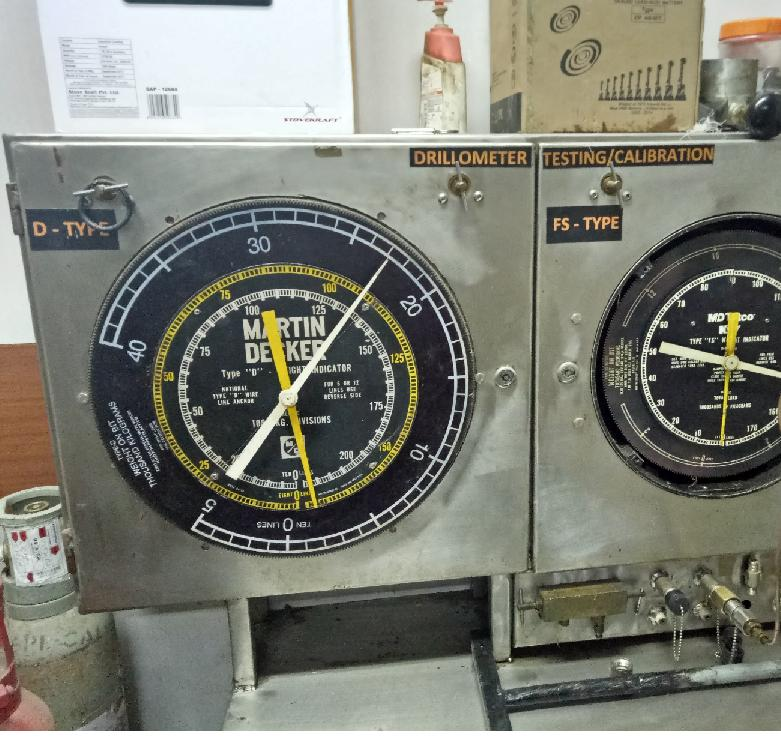
\includegraphics[scale=0.2]{images/drillometer}
\centering 
\caption{A Picture of Drillometer}
\end{figure}

\vspace{2em}


% However, most rigs are equipped with a
%weight indicator that has a second indicator dial that can be set to.
%read zero ("zeroed") with the drill string hanging free, and works
%backwards from the main indicator dial. After proper zeroing, any
%weight set on bottom (that takes weight away from the main dial), has
%the effect of adding weight to this secondary dial, so that the driller
%can read weight on bit directly from the dial.